\section{Konzept-unabhängige Funktionen}
Die Konzepte unterscheiden sich mechanisch, denn jedes einzelne Konzept verfolgt ein andere Idee um den Ball in den Korb zu befördern. Doch die Funktionen 'Bordcomputer', 'Kommunikation' und 'Ortung des Korbes' sind für alle vereinheitlicht. Jedes Konzept wird mit den gleichen konkreten Umsetzungen in diesen Bereichen ausgerüstet.

\subsection{Übersicht}
Auf der Grafik sieht man die gewählten Umsetzungen. In den nachfolgenden Kapitel sind diese begründet.

\begin{figure}[h!]
	\centering
	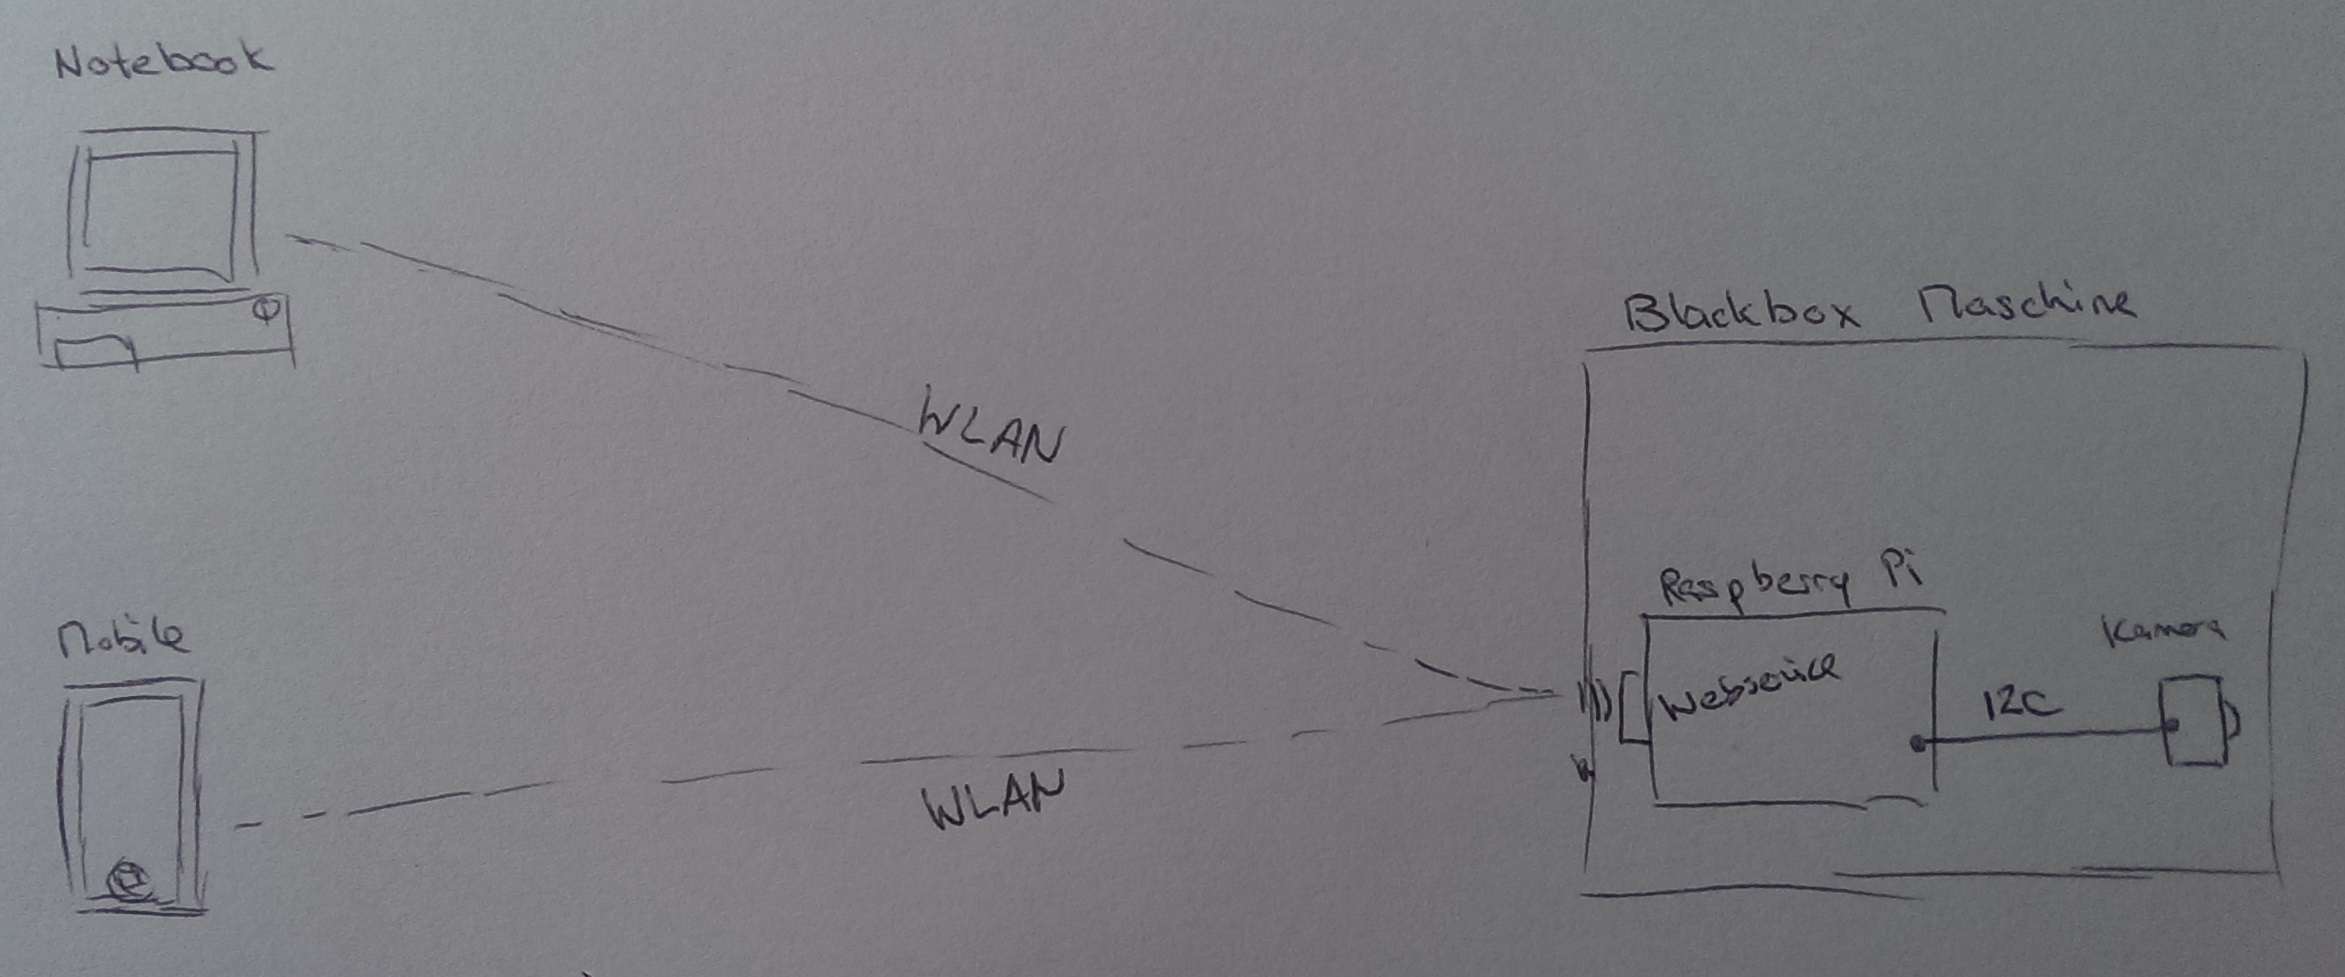
\includegraphics[scale=0.15]{../../fig/konzeptunabhaengige_funktionen_overview.jpg}
	\caption{Übersicht konzept-unabhängige Funktionen}
	\label{fig:konzept1}
\end{figure}

\subsection{Bordcomputer}
Der Einsatz eines Bordcomputer ist unabdingbar. Im Kapitel \ref{ssc_raspberry_pi} wird die Verwendung des 'Raspberry PIs' empfohlen. Kostengünstig, weit verbreitet und ein grosser Funktionsumfang sind schlagkräftige Argumente. Möglicherweise stellen sich Low-Level Operationen als möglicher Knackpunkt heraus. Für dieses Problem kann schnell auf einen 'Freedomboard FRDM-KL25Z' zugegriffen werden, welcher die Aufgaben übernehmen kann (siehe Abschnitt \ref{ssc_lowlevel_fallback}).

\subsection{Kommunikation}

Die präferierte Variante für die Kommunikation ist das Benutzen des WLANs. Sowohl auf Seite der Maschine steht mit dem Bordcomputer ein TCP/IP fähiges Geräte zur Verfügung. Auf der anderen Seite der Steuerungseinheit besitzt heute nahezu jedes Geräte TCP/IP (Notebooks, Mobile Devices). Als möglicher Fallback kann auch Bluetooth gewählt werden, dies aber nur, wenn einer der beiden Teilnehmer kein WLAN unterstützt (siehe Abschnitt \ref{sc_kommunikation}).
Die Kommunikation an sich war in den Versuchen kein Problem und konnten problemlos durchgeführt werden (siehe Anhang \ref{anhang-kommunikation}).

\subsection{Ortung des Korbes}
Bei der Ortung des Korbes wird auf Optik gesetzt. Denn die Versuche mit Ultraschall- sowie Lasermodulen waren nicht zufriedenstellend (siehe Abschnitt \ref{ssc_ortung_des_korbs}).
An dem 'Raspberry PI' kann eine Kamera angeschlossen werden. Das Bild wird entweder direkt auf dem 'Raspberry PI' ausgewertet oder an eine externe Einheit geschickt, welche die benötigte Rechenpower zur Verfügung stellt.
